\chapter{State of the Art and Theoretical Background}

\section{Introduction}
This chapter establishes the academic and theoretical foundation required to defend \projectname{} rigorously. The implemented platform is not only the result of practical integration between several tools; it is the consequence of architectural choices made under well-known constraints in distributed data engineering. For that reason, the chapter begins with global concepts and design trade-offs before moving toward architectural models. Its objective is to explain why a distributed customer-data platform must be designed in layers, why storage and compute cannot be treated as isolated concerns, and why governance, observability, and security are not optional additions but structural requirements.

The discussion is informed by the broader literature on distributed and data-intensive systems, including the design logic emphasized by Martin Kleppmann in \emph{Designing Data-Intensive Applications}, especially around reliability, scalability, maintainability, partitioning, replication, and consistency trade-offs. The goal is not to summarize the entire field, but to identify the concepts that directly justify the architecture adopted later in this report.

\section{Foundations of Modern Distributed Data Systems}

\subsection{From Centralized Systems to Distributed Data Platforms}
Traditional information systems were largely organized around centralized databases and a relatively small number of application servers. This model remains effective when data volume is moderate, operational contexts are stable, and the number of consumers remains limited. However, once organizations begin collecting heterogeneous data from multiple channels, centralized architectures become difficult to sustain. Storage pressure increases, computational workloads become more varied, and the system becomes more sensitive to single-node bottlenecks.

Distributed data platforms emerged as a response to these limitations. Their purpose is not only to increase raw capacity, but also to separate responsibilities according to operational logic. In a modern platform, event transport, raw storage, distributed computation, metadata management, analytical exposure, data quality validation, and observability can be handled by different services while still forming a coherent whole. This decomposition allows each concern to evolve with the technical model best suited to it.

Figure~\ref{fig:centralized-vs-distributed} summarizes this transition from a monolithic structure toward a layered distributed platform. It highlights the architectural shift from a single server concentrating ingestion, storage, processing, and access responsibilities to a distributed model in which ingestion, storage, compute, metadata, and analytical exposure are separated into specialized layers.

\begin{figure}[htbp]
    \centering
    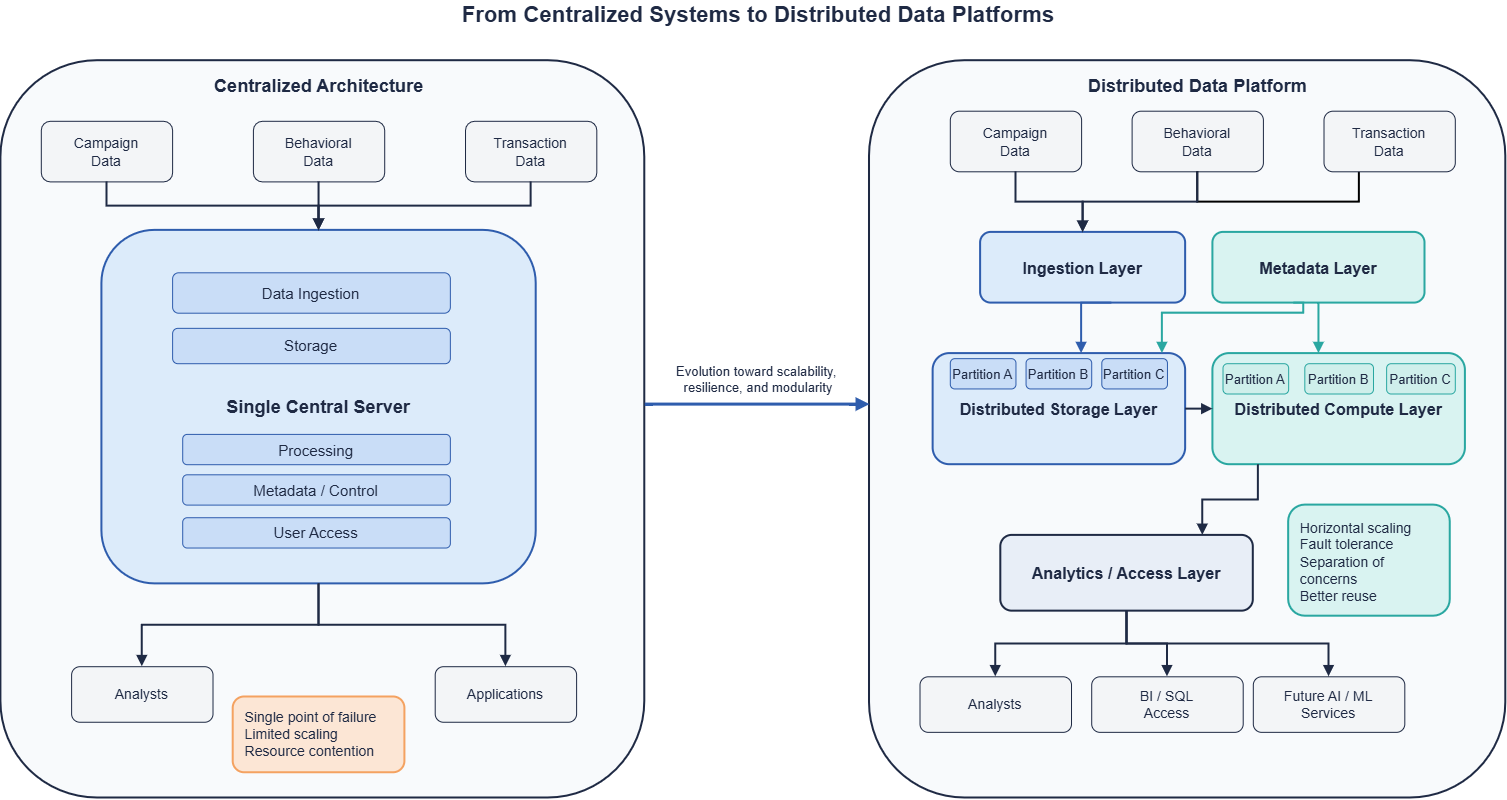
\includegraphics[width=\textwidth]{90_assets/figures/chapter_2/fig_2_1_centralized_vs_distributed.png}
    \caption{Conceptual evolution from centralized architectures to distributed data platforms.}
    \label{fig:centralized-vs-distributed}
\end{figure}

\subsection{Vertical Scaling vs Horizontal Scaling}
One of the first decisions in large-scale systems concerns how growth should be absorbed. Vertical scaling strengthens a machine by increasing CPU, memory, or storage capacity. It is often simpler in the short term because the system does not need to be partitioned immediately. Nevertheless, it has two major limits: physical growth is finite, and dependence on a small number of powerful machines weakens resilience.

Horizontal scaling increases capacity by adding nodes. This model is more complex because it requires workload distribution, coordination, and partial-failure management. However, it offers better long-term elasticity and better alignment with modern data engineering workloads. Storage can be distributed across nodes, compute can run in parallel, and replication strategies can reduce the risk of complete service interruption. For a distributed customer-data platform, horizontal scaling is therefore not just a performance technique; it is a structural architectural principle.

\subsection{Reliability, Scalability, and Maintainability}
The literature on distributed systems frequently emphasizes three central qualities: reliability, scalability, and maintainability. Reliability refers to the system's ability to continue providing correct service despite component failures, abnormal workloads, or operational disturbances. Scalability refers to the platform's capacity to grow without disproportionate degradation or redesign. Maintainability refers to the ability to understand, operate, extend, and debug the system over time.

These three qualities are fundamental for a platform such as \projectname. A customer-data foundation that is unreliable cannot support trusted analytical reuse. A platform that is not scalable cannot sustain new datasets, new clients, or future machine learning use cases. A platform that is not maintainable becomes fragile and difficult to defend academically because its behavior depends on hidden assumptions and manual intervention. Consequently, these qualities are not abstract ideals; they are direct evaluation criteria for the engineering relevance of the project.

\subsection{Data-Intensive Systems as a Distinct Engineering Problem}
Data-intensive systems differ from ordinary software systems because data movement, storage, replayability, and consistency become first-class engineering concerns. In such systems, correctness is not defined only by the logic of business functions. It also depends on whether data is durably persisted, whether transformations are reproducible, whether schemas remain interpretable over time, and whether the system can explain the origin and lifecycle of the information it exposes.

This distinction is important for the academic positioning of the present work. \projectname{} is not simply an application with a database behind it. It is a distributed data engineering platform whose value lies in organizing the lifecycle of heterogeneous customer-related data in a reliable, observable, and governable way. Therefore, the project must be understood through the conceptual framework of data-intensive and distributed systems.

\section{Core Theoretical Trade-offs in Distributed Data Engineering}

\subsection{The CAP Theorem and Consistency Trade-offs}
The CAP theorem remains one of the best-known conceptual references in distributed systems. It states that under network partition conditions, a distributed system cannot simultaneously provide both strong consistency and full availability. Although this statement is often simplified in practice, its educational importance is clear: once a system is distributed, architects must explicitly decide how consistency, availability, and failure tolerance are balanced.

For data platforms, this means that different layers of the architecture can make different trade-offs. Event transport systems, distributed filesystems, metadata services, and analytical table layers are not expected to behave identically. Some prioritize durability and replayability, others prioritize read scalability, and others introduce stronger transactional semantics for curated analytical datasets. The value of the theorem in the present context is therefore not to impose one universal answer, but to justify why a multi-layer architecture is necessary.

\subsection{ACID vs BASE Models}
ACID properties traditionally define the transactional expectations of strongly controlled database systems: atomicity, consistency, isolation, and durability. These properties are essential when every update must remain immediately and strictly correct. However, not every stage of a distributed data platform requires the same guarantees at the same time.

BASE, commonly summarized as Basically Available, Soft state, Eventual consistency, represents a different philosophy. It accepts temporary divergence and asynchronous convergence when this allows better distribution, availability, or throughput. Many ingestion and transport layers operate closer to BASE-like behavior, whereas curated analytical layers often benefit from stronger ACID-like semantics. This explains the importance of table formats and catalog layers that reintroduce stronger transactional guarantees on top of flexible distributed storage.

\subsection{Data Partitioning and Replication}
Partitioning divides data into smaller units so that storage and computation can be distributed across multiple nodes. It is one of the foundational mechanisms behind modern large-scale platforms. Without partitioning, a single node becomes a natural bottleneck for read throughput, write throughput, fault recovery, and transformation execution.

Replication complements partitioning by improving resilience and availability. When multiple copies of data or logs exist, the system can continue operating even when one node is degraded or unavailable. Yet replication is not free: it introduces coordination overhead and consistency challenges. This is why partitioning and replication should not be viewed as purely implementation-level details. They are fundamental architectural instruments for balancing scale, resilience, and operational complexity.

\subsection{Fault Tolerance and Service Resilience}
In distributed systems, failure must be considered normal rather than exceptional. Nodes may disappear, ports may become temporarily unavailable, certificates may expire, services may start in the wrong order, and storage volumes may create cascading readiness issues. A resilient platform therefore needs explicit strategies for retries, health checks, replication, recovery, and replay.

This principle is particularly relevant in data engineering because failures can affect not only uptime but also data trust. A silent ingestion failure may result in missing data. A metadata failure may make tables unreadable. A readiness misconfiguration may cause an orchestration layer to fail even when the data itself is correct. Therefore, fault tolerance is directly tied to platform credibility and reproducibility.

\subsection{Batch Processing vs Stream Processing}
Batch processing is based on finite datasets processed periodically or on demand. It is suitable for historical backfills, curated analytical transformations, and reproducible large-scale recomputation. Stream processing is based on continuous flows of records or events that are handled incrementally as they arrive. It is useful when ingestion or propagation must remain closer to real-time behavior.

These two paradigms should not be treated as mutually exclusive. In modern platforms, they often coexist. Event streaming can capture and transport raw information continuously, while downstream computation may structure the resulting data into trusted analytical tables through batch or micro-batch logic. This hybrid view is especially relevant in customer-data engineering, where event freshness matters but governance and curated analytical reuse remain essential.

\subsection{Schema-on-Write vs Schema-on-Read}
Schema-on-write means that data must be shaped according to a predefined structure before it is stored in an authoritative analytical repository. This approach improves control and downstream semantic stability, but it may reduce ingestion flexibility. Schema-on-read, by contrast, stores raw or semi-structured data first and interprets structure later when the data is processed or queried.

This trade-off is central to modern lakehouse thinking. Raw layers benefit from schema-on-read because they preserve source fidelity and support replay. Curated layers benefit from stronger schema discipline because users require stable and understandable analytical entities. A layered data platform therefore does not simply choose one strategy over the other. It combines them in sequence, using flexibility for raw persistence and stronger structure for curated consumption.

\section{Big Data Foundations}

\subsection{The Five Vs of Big Data}
Big Data is often introduced through five dimensions: volume, velocity, variety, veracity, and value. Volume refers to the quantity of data that must be managed. Velocity refers to the rate at which data is generated and moved. Variety refers to the diversity of formats, structures, and source semantics. Veracity concerns the reliability and quality of the data. Value concerns the usefulness that can be extracted from it for decision-making and future intelligent services.

These dimensions remain relevant because they show that data engineering complexity does not depend only on scale. Even when data volume remains manageable, high variety, high reuse pressure, and high governance expectations can justify a distributed architecture. This is particularly true for customer-data platforms, where datasets often differ in structure, semantics, and analytical purpose.

\subsection{Heterogeneous Data Sources and Data Variety}
Customer understanding rarely comes from a single operational system. It may involve campaign response datasets, online behavioral signals, e-commerce or retail transactions, session-level intent indicators, and profile-related attributes. Each source differs in format, cadence, completeness, and downstream meaning. This heterogeneity makes integration difficult because technical normalization is not sufficient; semantic reconciliation is also required.

As a result, variety becomes both a storage problem and a modeling problem. The platform must be able to ingest different raw forms, persist them durably, and later organize them into analytical layers without erasing their provenance. This is one of the strongest arguments for using layered architecture rather than directly forcing all incoming data into one rigid warehouse model.

\subsection{Distributed Storage Principles}
Distributed storage spreads persisted data across multiple nodes instead of concentrating it on a single machine. Its goals include capacity growth, resilience, replication, parallel read/write support, and better alignment with distributed compute. An important consequence of distributed storage is that it separates durable raw persistence from the compute jobs that later transform the data.

This separation has strong academic value. When raw data is durably preserved, pipelines become replayable and easier to audit. Transformations can be rerun without repeatedly depending on the original upstream source. The raw layer therefore serves both operational recovery and methodological reproducibility. In a PFE context, this is a strong argument because it shows that architecture supports not only execution but also traceable engineering reasoning.

\subsection{Distributed Compute Principles}
Distributed compute allows processing tasks to be decomposed and executed across several nodes. Instead of one machine reading and transforming an entire dataset, work is split according to partitions, files, or execution stages. This can reduce total execution time and align compute more closely with distributed storage.

However, distributed compute is beneficial only when the workload justifies it. Task scheduling, serialization, dependency management, and cluster readiness all introduce overhead. Therefore, an academically defensible platform must show that distributed compute is not used only as a slogan. It must be used where the problem structure, data movement pattern, and storage organization make parallel execution meaningful.

\section{Evolution of Analytical Data Architectures}

\subsection{Traditional Data Warehouse Architecture}
The traditional data warehouse is organized around structured, curated, and strongly modeled analytical data. It is highly effective for stable reporting, dimensional modeling, and SQL-based decision support. Its main strength is semantic control.

Its limitation appears when heterogeneous or semi-structured data must be ingested rapidly and preserved before full normalization. In such contexts, the warehouse-only model can become too rigid because it expects analytical structure too early in the lifecycle. This rigidity is often incompatible with modern customer-data environments where raw preservation and later reinterpretation are valuable.

\subsection{Data Lake Architecture}
The data lake emerged as a response to the rigidity of traditional warehouses. It enables large quantities of raw and semi-structured data to be stored before full modeling. This increases ingestion flexibility and supports exploratory reuse across different downstream consumers.

However, data lakes also introduced a new risk: if metadata, naming discipline, and validation remain weak, the platform can degrade into an opaque storage zone with low analytical trust. In other words, the lake model solves flexibility problems but can create governance problems. This is why the data lake alone is rarely sufficient for a mature customer-data platform.

\subsection{Data Lakehouse Architecture}
The data lakehouse seeks to combine the flexibility of the lake with the transactional and governance discipline associated with warehouses. It preserves distributed and replayable storage logic while adding stronger table semantics, better schema evolution control, and improved analytical exposure.

This model is particularly well adapted to projects such as \projectname. It allows raw datasets to be preserved in distributed storage while curated datasets are exposed through governed tables suitable for transformation frameworks and SQL query engines. The lakehouse can therefore be defended as an architectural response to the need for both flexibility and trust.

\subsection{Lambda Architecture}
Lambda architecture organizes processing through two paths: a batch path for full historical recomputation and a speed layer for low-latency updates. Its objective is to reconcile correctness and freshness. The model was influential because it formalized the difficulty of satisfying both needs through a single pipeline.

Nevertheless, Lambda architecture is often criticized for operational duplication. Two processing logics must be maintained, monitored, and reconciled. Its academic relevance remains high because it helps explain why organizations later looked for simplified architectures able to keep event responsiveness without multiplying engineering burden.

\subsection{Kappa Architecture}
Kappa architecture reduces the conceptual duplication of Lambda by emphasizing a stream-centered approach in which the event log becomes the main source of truth. Reprocessing is achieved through replay rather than through a separate batch computation layer.

This model is attractive when event logs are rich, retention is strong, and the platform is comfortable treating stream replay as its main recovery and recomputation mechanism. However, many real analytical platforms still require clearly governed historical layers and structured table abstractions. Therefore, Kappa is instructive, but not automatically sufficient for every customer-data use case.

\subsection{Comparative Analysis of These Architectures}
The historical movement from warehouses to lakes, from lakes to lakehouses, and from isolated reporting toward event-aware architectures reflects a broader shift in priorities. Early architectures privileged control and stable relational semantics. Later architectures privileged ingestion flexibility and scale. Contemporary platforms increasingly seek a hybrid answer that preserves raw fidelity, enables distributed processing, and still produces governed analytical products.

For \projectname, the lakehouse model is the most suitable. It supports raw bronze persistence, distributed storage, structured analytical tables, metadata-driven reuse, and downstream SQL exploration. It also remains compatible with event-driven ingestion patterns and security hardening requirements. As a result, the selected architecture is not arbitrary; it is a reasoned synthesis of the state of the art.

\section{Foundational Concepts for Governance and Trust in Data Platforms}

\subsection{Metadata, Cataloging, and Data Discovery}
Metadata gives meaning to stored data by describing structure, origin, semantics, and technical location. Without metadata, even accessible data can remain practically unusable. Cataloging extends this principle by making datasets discoverable and interpretable by different actors.

In a distributed customer-data platform, metadata is especially important because the architecture spans several services and layers. Governance cannot depend on informal memory alone. A defensible platform must therefore treat schema registration, table visibility, and dataset discovery as explicit capabilities.

\subsection{Data Lineage and Traceability}
Lineage refers to the ability to trace how data moved from source to output, which transformations were applied, and which downstream assets depend on which upstream artifacts. Traceability is essential for reproducibility, debugging, and auditability.

From an academic point of view, lineage helps distinguish a genuine data engineering platform from a simple collection of disconnected scripts. When lineage can be reconstructed, the platform becomes explainable. This is essential for a PFE project that must defend not only outcomes but also the logic by which those outcomes were produced.

\subsection{Data Quality Dimensions}
Data quality is multidimensional. Common dimensions include completeness, consistency, validity, accuracy, timeliness, and uniqueness. These dimensions are especially important in customer-data contexts because downstream segmentation, profiling, or future predictive analytics become weak when source data is inconsistent or poorly governed.

Modern platforms increasingly formalize quality as an explicit layer of the architecture rather than as a purely manual cleaning activity. Checks, expectations, thresholds, and validation artifacts transform quality into a monitored engineering property. This move is important because it makes trust operationally visible.

\subsection{Observability in Distributed Data Systems}
Observability is the capacity to infer the internal state of a system through emitted evidence such as metrics, logs, traces, health checks, and runtime indicators. In distributed environments, observability is crucial because failures often emerge from the interaction between components rather than from one isolated service.

For data engineering, observability is tightly linked to platform trust. If the system cannot show whether ingestion succeeded, whether storage is healthy, whether services are reachable, or whether transformations produced expected results, its outputs become difficult to defend. Observability is therefore part of the platform's academic credibility as well as its operational practicality.

\section{Security Foundations for Distributed Data Platforms}

\subsection{Authentication in Distributed Systems}
Authentication establishes who a user or service is. In distributed environments, it becomes critical because communication crosses process, host, and network boundaries. Storage services, metadata layers, and query endpoints must be able to distinguish legitimate principals from unauthorized ones.

Without strong authentication, a distributed platform depends on implicit trust between components, which becomes increasingly dangerous as the number of services grows. Therefore, authentication is a structural foundation of secure distributed data engineering.

\subsection{Authorization and Access Control}
Once identity is established, the system must determine which actions are permitted. Authorization controls access to services, datasets, administrative operations, and query interfaces. It operationalizes the principle of least privilege by restricting each actor to the minimum access necessary for its role.

In data platforms, authorization cannot be limited to end-user interfaces alone. It also applies to service-to-service calls, operational scripts, metadata access, and internal gateways. A mature distributed architecture must therefore combine authentication and authorization rather than treating them as separate afterthoughts.

\subsection{Encryption in Transit and Encryption at Rest}
Encryption in transit protects data while it moves between nodes, services, or users. It reduces exposure to interception and helps preserve confidentiality across the network. Encryption at rest protects persisted data on storage media and reduces exposure if storage devices or mounted runtime paths are accessed outside intended controls.

These two mechanisms answer different threat surfaces and must be treated as complementary. In a multi-service lakehouse platform, data frequently moves through ingestion, orchestration, query, and monitoring channels. Consequently, transport security and persistent storage protection both belong to the theoretical foundation of a defensible architecture.

\subsection{Secure Service Exposure in Multi-Node Environments}
Distributed platforms expose numerous service endpoints: orchestration UIs, query interfaces, storage consoles, monitoring dashboards, and service APIs. If these are exposed without proxying, credential checks, and transport protection, the system accumulates a wide attack surface.

Secure exposure therefore requires deliberate control of entry points, certificates, internal-versus-external interfaces, and service-access boundaries. This is particularly relevant to \projectname{} because one of its core challenges is not only to run multiple services, but to expose them in a way that remains manageable, authenticated, and defensible.

\section{Positioning of the Present Work}

\subsection{Theoretical Alignment with Distributed Lakehouse Principles}
The architecture of \projectname{} aligns with distributed lakehouse principles because it separates raw ingestion, distributed persistence, curated analytical structuring, metadata management, validation, orchestration, and observability into coordinated layers. This layered model directly reflects the theoretical distinctions discussed earlier in the chapter: flexible raw persistence, stronger structure for trusted curated layers, distributed compute for transformation, and governance for analytical reuse.

\subsection{Why This Project Is a Data Engineering Platform and Not a Final AI Product}
Although the broader \initiative{} initiative may later incorporate advanced analytical and intelligent marketing functions, the present work should not be described as a completed AI product. Its implemented contribution lies in the design and deployment of the distributed data platform that makes future analytics possible under reproducible, governed, and secure conditions.

This distinction is academically essential. It prevents exaggerated claims and keeps the defense aligned with the real contribution of the project: distributed storage, distributed processing, analytical structuring, data quality control, orchestration, monitoring, and infrastructure hardening. These are substantial engineering results in their own right.

\subsection{Positioning of AdOptimizer CDP within AdOptimizer AI}
Within \initiative, \projectname{} plays the role of the distributed customer-data foundation. It is the technical layer responsible for receiving heterogeneous inputs, organizing them into replayable and structured movement patterns, persisting them durably, curating them into analytical datasets, and exposing them to future consumers under controlled conditions.

This positioning gives the project a clear strategic identity. It is neither an isolated classroom exercise nor a finished business intelligence product. It is a concrete infrastructure contribution embedded in a larger company initiative while remaining academically defensible as a modern Big Data and Data Engineering platform.

\section{Conclusion}
This chapter established the theoretical and architectural background that justifies the design of \projectname. It introduced the evolution of distributed data systems, the principal engineering trade-offs that shape them, the foundations of Big Data platforms, the comparative logic of modern analytical architectures, and the core principles of governance, observability, and security in distributed environments.

On this basis, the following chapters can now move from theory to requirements, design, and implementation. The platform can therefore be presented not as a collection of tools, but as a coherent response to well-identified distributed data engineering challenges.
